\section{Ανάλυση συστήματος}
Σε αυτό το εργαστήριο καλούμαστε να εφαρμόσουμε γραμμική ανάδραση καταστάσεων στο σύστημά μας σύμφωνα με τις παραμέτρους που υπολογίσαμε στο 1\textsuperscript{ο} εργαστήριο.

\makeatletter
\newcommand{\xRightarrow}[2][]{\ext@arrow 0359\Rightarrowfill@{#1}{#2}}
\makeatother
\newcommand\numberthis{\addtocounter{equation}{1}\tag{\theequation}}
\newcommand{\kone}{\frac{-k_m}{T_m s + 1}}
\newcommand{\ktwo}{k_{\mu}}
\newcommand{\kthree}{\frac{k_0}{s}}
\begin{figure}[htb]
    \centering
    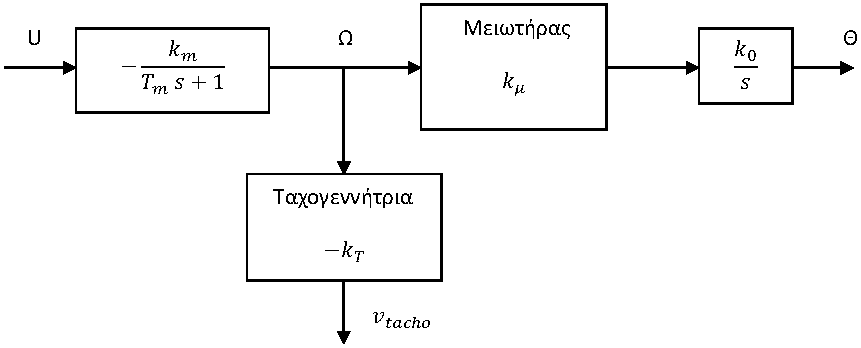
\includegraphics[width=\linewidth]{system}
    \caption{Το δομικό διάγραμμα του συστήματος στο οποίο εργαζόμαστε}
    \label{fig:system}
\end{figure}

\begin{figure}[htb]
    \centering
    {
\tikzstyle{block} = [draw, rectangle, minimum height=3em]
\tikzstyle{sum} = [draw, fill=blue!20, circle, node distance=1cm]
\tikzstyle{input} = [coordinate]
\tikzstyle{output} = [coordinate]
\tikzstyle{pinstyle} = [pin edge={to-,thin,black}]

% 12cm calculated with inkscape.
\begin{tikzpicture}[auto, scale=\linewidth/12cm, transform shape, node distance=2cm,>=latex']
    % We start by placing the blocks
    \node [input, name=input] {};
    \node [block, right of=input] (k_r) {$k_r$};
    \node [sum, right of=k_r] (sum) {$+$};
    \node [block, right of=sum, node distance=3.5cm] (controller1) {$\kone$};
    \node [block, right of=controller1, node distance=2.5cm] (controller2) {$\ktwo$};
    \node [block, right of=controller2, node distance=1cm] (controller3) {$\kthree$};
    \draw [->] (controller1) -- node[name=Omega] {$\Omega$} (controller2);
    \node [output, right of=controller3] (output) {};
    \node [block, below of=controller1] (k_tacho) {$-k_T$};
    \node [block, left of=k_tacho, node distance=2.2cm] (k2) {$k_2$};
    \node [block, below of=k2] (k1) {$k_1$};
    \node [sum] (sumbelow) at (k2 -| sum) {$+$};

    % Once the nodes are placed, connecting them is easy.
    \draw [draw,->] (input) -- node {$r$} (k_r);
    \draw [draw,->] (k_r) -- node {$+$} (sum);
    \draw [->] (sum) -- node {$e$} (controller1);
    \draw [->] (controller2) -- node {} (controller3);
    \draw [->] (controller3) -- node [name=theta] {$x_1 = \theta$}(output);
    \draw [->] (Omega) |- (k_tacho);
    \draw [->] (k_tacho) -- node[label={[below]$x_2$}, label={$v_{tacho}$}] {} (k2);
    \draw [->] (theta) |- (k1);
    % Second sum node.
    \draw [->] (k1) -| node[pos=0.9] {$+$} node [near end] {} (sumbelow);
    \draw [->] (k2) -- node[pos=0.9] {$+$} node [near end] {} (sumbelow);
    \draw [->] (sumbelow) -- node[pos=0.9] {$-$} node [near end] {} (sum);
\end{tikzpicture}
}

    \caption{Το σύστημα με γραμμική ανάδραση}\label{fig:system-feedback}
\end{figure}

Από το σχήμα~\ref{fig:system-feedback}:
\begin{align*}
    e \cdot{} \frac{-k_m}{T_m s + 1} & = \Omega \\
    \Omega \cdot{} (-k_T)            & = x_2
\end{align*}
πολλαπλασιάζοντας:
\begin{equation*}
    e \cdot{} \frac{k_m k_T}{T_m s + 1} = x_2 \implies e k_m k_T = T_m s x_2 + x_2
\end{equation*}
όμως ισχύει:
\begin{align*}
    \dot{x}_2 & = s x_2                     \\
    e         & = k_r r - k_1 x_1 - k_2 x_2
\end{align*}
άρα:
\begin{align*}
    T_m \dot{x}_2 & = (k_r r - k_1 x_1 - k_2 x_2) k_m k_T - x_2 \implies                                                                   \\
    \dot{x}_2     & = -\frac{k_1 k_m k_T}{T_m} x_1 - \frac{1 + k_2 k_m k_T}{T_m} x_2 + \frac{k_r k_m k_T}{T_m} r \numberthis\label{eq:dx2}
\end{align*}
Για το $\dot{x}_1$ ισχύει:
\begin{align*}
    x_1       & = k_{\mu} k_0 \frac{\Omega}{s} \xRightarrow{\Omega = -\frac{1}{k_T} x_2} \\
    s x_1     & = -\frac{k_{\mu} k_0}{k_T} x_2 \implies                                  \\
    \dot{x}_1 & = -\frac{k_{\mu} k_0}{k_T} x_2 \numberthis\label{eq:dx1}
\end{align*}
Στη τελική κατάσταση θέλουμε $\dot{x}_1 = x_2 = \ddot{x}_2 = 0$ και $x_1 = \theta_{ref}$ έτσι:
\begin{align*}
    - \frac{k_1 k_m k_T}{T_m} x_1 - \frac{1 + k_2 k_m k_T}{T_m} x_2 + \frac{k_r k_m k_T}{T_m} r & = 0 \implies                      \\
    k_r                                                                                         & = k_1 \numberthis\label{eq:kr-k1}
\end{align*}
Το τελικό σύστημα από~\ref{eq:dx2},~\ref{eq:dx1} και~\ref{eq:kr-k1}:
\begin{align}
    \dot{x}_1 & = -\frac{k_{\mu} k_0}{k_T} x_2                                                               \\
    \dot{x}_2 & = -\frac{k_1 k_m k_T}{T_m} x_1 - \frac{1 + k_2 k_m k_T}{T_m} x_2 + \frac{k_1 k_m k_T}{T_m} r
\end{align}
ή σε μορφή πίνακα:
\begin{equation}
    \dot{x} = A x + b r
\end{equation}
όπου
\begin{align}
    A & = \begin{bmatrix}
        0                        & -\frac{k_{\mu} k_0}{k_T}    \\
        -\frac{k_1 k_m k_T}{T_m} & \frac{1 + k_2 k_m k_T}{T_m}
    \end{bmatrix} \\
    B & = \begin{bmatrix}
        0                       \\
        \frac{k_1 k_m k_T}{T_m}
    \end{bmatrix}
\end{align}
Η χαρακτηριστική εξίσωση προκύπτει:
\begin{align*}
\abs{s I - A} &= 0 \implies\\
s^2 + \frac{1 + k_2 k_m k_T}{T_m} s - \frac{k_0 k_1 k_{\mu} k_m}{T_m} &= 0\numberthis
\end{align*}
Έτσι, για επιθυμητό πολυώνυμο
\begin{equation}
p_d(s) = s^2 + a_1 s + a_2\label{eq:desired}
\end{equation}
έχουμε
\begin{alignat}{3}
a_1 &= \frac{1 + k_2 k_m k_T}{T_m} &\implies k_2 &= \frac{a_1 T_m - 1}{k_m k_T}\\
a_2 &= - \frac{k_0 k_1 k_{\mu} k_m}{T_m} &\implies k_1 &= \frac{-a_2 T_m}{k_0 k_{\mu} k_m}
\end{alignat}
Αυτά τα κέρδη θα χρησιμοποιήσουμε για τον έλεγχο του συστήματός μας.
Οι τιμές των $a_1$, $a_2$ προκύπτουν από τις σχέσεις:
\begin{align}
a_1 &= 2 \zeta \omega_n\\
a_2 &= {\omega_n}^2
\end{align}
όπου πρέπει να επιλεγούν οι τιμές των $\zeta$, $\omega_n$ σύμφωνα με τις απαιτήσεις μας για το σύστημα.
